\documentclass[
    % -- opções da classe memoir --
    12pt,               % tamanho da fonte
    openright,          % capítulos começam em pág ímpar (insere página vazia caso preciso)
    %twoside,            % para impressão em verso e anverso. Oposto a oneside
    oneside,
    a4paper,            % tamanho do papel.
    %chapter=TITLE,     % títulos de capítulos convertidos em letras maiúsculas
    %section=TITLE,     % títulos de seções convertidos em letras maiúsculas
    %subsection=TITLE,  % títulos de subseções convertidos em letras maiúsculas
    %subsubsection=TITLE,% títulos de subsubseções convertidos em letras maiúsculas
    % -- opções do pacote babel --
    english,            % idioma adicional para hifenização
    brazil           % o último idioma é o principal do documento
    ]{ufscar-sc}

\usepackage{graphicx} % Imagem com subimagens
\usepackage{subcaption} % Imagem com subimagens
\usepackage{float} % Forçar posicionamento das imagens

% ---
% Pacotes básicos
% ---
\usepackage{lmodern}            % Usa a fonte Latin Modern
\usepackage[T1]{fontenc}        % Selecao de codigos de fonte.
\usepackage[utf8]{inputenc}     % Codificacao do documento (conversão automática dos acentos)
% ---

% ---
% Pacotes adicionais, usados apenas no âmbito do Modelo Canônico do abnteX2
% ---
\usepackage{lipsum}             % para geração de dummy text
\usepackage{blindtext}          % para geração de dummy text

% ---

% ---
% CONFIGURAÇÕES DE PACOTES ADICIONAIS UTEIS
% ---
\usepackage{pdfpages}			% para incluir arquivos pdf no documento
%\usepackage[final,obeyFinal]{todonotes}			% para não imprimir pendencias na versão final

\usepackage[printonlyused]{acronym}		% siglas


% ---
% Informações de dados para CAPA e FOLHA DE ROSTO
% ---
\titulo{Experimento 02 - Implementação de um meio-somador e uso de um display de 7 segmentos
como dispositivo de saída}

% Trabalho individual
%\autor{AUTOR DO TRABALHO}

% Trabalho em Equipe
% ver também https://github.com/abntex/abntex2/wiki/FAQ#como-adicionar-mais-de-um-autor-ao-meu-projeto
\renewcommand{\imprimirautor}{
\begin{tabular}{lr}
Joao Vitor Azevedo Marciano & 743554 \\
Lorhan Sohaky de Oliveira Duda Kondo & 740951 \\
\end{tabular}
}


\departamento{Departamento de Computação}
\curso{Ciência da Computação}
\disciplina{Laboratório de Circuitos Digitais}

\preambulo{}

\local{São Carlos - SP}
\data{\the\year}

% Definir o que for necessário e comentar o que não for necessário
% Utilizar o Nome Completo
\orientador{Fredy João Valente}

\instituicao{%
  \imprimirifsp
  \par
  \imprimirdepartamento
  \par
  \imprimircurso
  \par
  \imprimirdisciplina
}

% ---


% ---
% Configurações de aparência do PDF final

% alterando o aspecto da cor azul
\definecolor{blue}{RGB}{41,5,195}

% informações do PDF
\makeatletter
\hypersetup{
        %pagebackref=true,
        pdftitle={\@title},
        pdfauthor={\@author},
        pdfsubject={\imprimirpreambulo},
        pdfcreator={LaTeX with abnTeX2},
        pdfkeywords={abnt}{latex}{abntex}{abntex2}{trabalho acadêmico},
        colorlinks=true,            % false: boxed links; true: colored links
        linkcolor=blue,             % color of internal links
        citecolor=blue,             % color of links to bibliography
        filecolor=magenta,              % color of file links
        urlcolor=blue,
        bookmarksdepth=4
}
\makeatother
% ---

% ---
% Espaçamentos entre linhas e parágrafos
% ---

% O tamanho do parágrafo é dado por:
\setlength{\parindent}{1.3cm}

% Controle do espaçamento entre um parágrafo e outro:
\setlength{\parskip}{0.2cm}  % tente também \onelineskip

% ---
% compila o indice
% ---
\makeindex
% ---


% ----
% Início do documento
% ----
\begin{document}

% Retira espaço extra obsoleto entre as frases.
\frenchspacing

\newpage

% ----------------------------------------------------------
% ELEMENTOS PRÉ-TEXTUAIS
% ----------------------------------------------------------
\pretextual

% ---
% Capa
% ---
\imprimircapa

% ---
% Folha de rosto
% (o * indica que haverá a ficha bibliográfica)
% ---
\imprimirfolhaderosto
%\imprimirfolhaderosto*
% ---


% ---
% inserir lista de ilustrações
% ---
\pdfbookmark[0]{\listfigurename}{lof}
\listoffigures*
\cleardoublepage
% ---

% ---
% inserir lista de tabelas
% ---
\pdfbookmark[0]{\listtablename}{lot}
\listoftables*
\cleardoublepage
% ---

% ---
% inserir lista de quadros
% ---
\pdfbookmark[0]{\listofquadrosname}{loq}
\listofquadros*
\cleardoublepage
% ---

% ---
% inserir lista de abreviaturas e siglas
% ---

% Utilizando acronym para tratar a apresentação de siglas e abntex para fazer a lista
% \item para abntex
% \acrodef para acronym
% o padrão da classe acronym é somente listas as siglas em uso, já o abntex vai listar todas definidas.

% a lista deve ser definida em ordem alfabética pois o abntex não ordena automaticamente

\newcommand{\sigla}[3]{\item[#2] #3
\acrodef{#1}[#2]{#3}\index{#2}}

\begin{siglas}
	\sigla{ci}{CI}{Circuito Integrado}
	\sigla{fpga}{FPGA}{\emph{Field Programmable Gate Array} - Arranjo de Portas Programáveis em Campo}
\end{siglas}



% ---


% ---
% inserir lista de símbolos
% ---
\begin{simbolos}
  \item[$ \Gamma $] Letra grega Gama
  \item[$ \Lambda $] Lambda
  \item[$ \zeta $] Letra grega minúscula zeta
  \item[$ \in $] Pertence
\end{simbolos}
% ---



% ---
% inserir o sumario
% ---
\pdfbookmark[0]{\contentsname}{toc}
\tableofcontents*
\cleardoublepage
% ---


% ----------------------------------------------------------
% ELEMENTOS TEXTUAIS
% ----------------------------------------------------------
\textual

% Para facilitar a manutenção é sempre melhore criar um arquivo por capitulo, para exemplo isso não é necessário
\chapter{Resumo}
	O experimento tem como objetivo implementar uma máquina de estado que corresponda ao
	funcionamento de uma porta giratório de banco. Confome a seguinte descrição:

	\begin{quotation}
		Considere uma porta giratória integrada com detector de metais, utilizada em bancos e
		desenvolva um projeto de um circuito Lógico Digital para Controle da porta utilizando FSM
		(máquina de estados finitos). A porta possui sensores de detecção de sentido de giro, detecção
		de presença de pessoas, sensor detecção de presença de metais para quem estiver entrando,
		sinalizador luminoso para luz verde (seguir em frente) e vermelho (retornar e colocar metais na
		janela lateral), além de mensagem sonora indicando a necessidade de voltar e retirar metais dos
		bolsos e colocar na janela lateral. Considere as seguintes características operacionais:
		A porta é bidirecional:
		1. Quando uma pessoa adentrar a porta giratória para sair ou para entrar deve ter o sensor
		de presença detecta a presença de pessoa no lado correspondente e acende uma luz
		verde para sinalizar o “vá em frente”;
		2. Se houver pessoas de ambos lados a preferência será para quem estiver saindo, assim
		deverá ser sinalizado verde de um lado (saída) e vermelho do lado entrada;
		3. A detecção de metais ocorrerá somente para quem estiver entrando, e em caso positivo,
		a porta deverá acender a luz vermelha e disparar mensagem audível para que a pessoa
		retorne e coloque metais na janela lateral;
		4. A porta deverá permanecer travada enquanto houver 2 pessoas simultâneas tentando
		entrar / sair, até que a pessoa entrando recue para aquela que estiver saíndo sair antes
		dela.
	\end{quotation}

	Para desenvolver tal projeto, dividiu-se a tarefa em etapas:
	\begin{enumerate}
	   \item Desenhar a máquina de estado para o cenário em questão;
	   \item Escrever um código Verilog para a máquina de estado no passo anterior;
	   \item Executar o código na \ac{fpga} e simulação.
	 \end{enumerate}

%Apresentar  o  objetivo  do  experimento e  sua  relação  com  o  mundo  real.
%Citar exemplos  de  produtos  e  dados  de  empresas  que  usam  circuitos  semelhantes.
%Dados  históricos  e  estatísticos,  em  temas  próximos,  são  desejáveis.
%Adicionar referências bibliográficas.

% Para facilitar a manutenção é sempre melhore criar um arquivo por capitulo, para exemplo isso não é necessário

%---------------------------------------------------------------------------------------
\chapter{Descrição da execução do experimento}

\section{Cenario 1}

	Foram necessários para o desenvolvimento do experimento:
	\begin{itemize}
		\item Multímetro Digital
		\item \ac{ci} de portas lógicas \textit{AND} ( \textit{datasheet} 7400 )
		\item \ac{ci} de portas lórigas \textit{OR}
		\item \ac{ci} de porta lógica inversora / \textit{NOT}( \textit{datashee} 7404)
		\item \textit{Protoboard}
		\item Fios para conectar as portas
		\item Fonte de Alimentação DC 5V
		\item LED Vermelho
		\item LED Verde
		\item 2 resistores para polarizar os LED’s
		\item Alicate
	\end{itemize}

	A partir do problema proposto, montou-se a seguinte expressão lógica
	$$ P . ( F + C + O) + (F . C . O)$$

	com P representando \textit{o voto do presidente}, F
	\textit{o voto do diretor financeiro}, C
	\textit{o voto do controller} e O \textit{o voto do diretor de operações}, após a
	montagem da expressão, foi elaborada a \autoref{table:tabelaVerdade1}. Com esta tabela e a expressão lógica,
	elaborou-se o circuito, conforme a \autoref{fig:desenhoCircuito1}. Com tais informações, foi repassado o circuito
	para o Quartus, depois renomeou-se as entradas e saídas para que, por meio do arquivo tradutor, a placa
	\ac{fpga} reconhecesse os componentes, conforme \autoref{fig:printCircuito1}.

	\begin{table}[h]
		\centering
		\caption{Tabela verdade da expressão lógica}\label{table:tabelaVerdade1}
		\begin{tabular}{c|c|c|c|c}
		%\hline
			\textbf{P} & \textbf{F} & \textbf{C} & \textbf{O} & \textbf{P.(F+C+O)+(F.C.O)} \\
			\hline
			0 & 0 & 0 & 0 & 0\\\hline
			0 & 0 & 0 & 1 & 0\\\hline
			0 & 0 & 1 & 0 & 0\\\hline
			0 & 0 & 1 & 1 & 0\\\hline
			0 & 1 & 0 & 0 & 0\\\hline
			0 & 1 & 0 & 1 & 0\\\hline
			0 & 1 & 1 & 0 & 0\\\hline
			0 & 1 & 1 & 1 & 1\\\hline
			1 & 0 & 0 & 0 & 1\\\hline
			1 & 0 & 0 & 1 & 1\\\hline
			1 & 0 & 1 & 0 & 1\\\hline
			1 & 0 & 1 & 1 & 1\\\hline
			1 & 1 & 0 & 0 & 1\\\hline
			1 & 1 & 0 & 1 & 1\\\hline
			1 & 1 & 1 & 0 & 1\\\hline
			1 & 1 & 1 & 1 & 1\\\hline

		\end{tabular}
	\end{table}

	\begin{figure}[H]
		\centering
		\caption{\label{fig:desenhoCircuito1}Desenho do circuito}
		\includegraphics[width=1\textwidth]{img/cenario1/desenhoCircuito}
	\end{figure}

	\begin{figure}[H]
		\centering
		\caption{\label{fig:printCircuito1}Imagem do circuito no Quartus}
		\includegraphics[width=1\textwidth]{img/cenario1/desenhoCircuito}
	\end{figure}

	\begin{figure}[H]
		\centering
		\caption{\label{fig:protoboard1}Configuração onde o LED Verde deveria acender (1001, por exemplo)}
		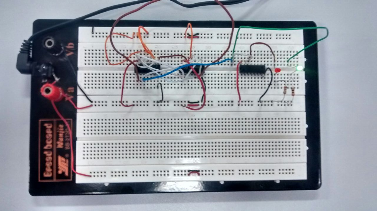
\includegraphics[width=1\textwidth]{img/cenario1/protoboard1}
	\end{figure}

	\begin{figure}[H]
		\centering
		\caption{\label{fig:protoboard2}Configuração onde o LED Vermelho deveria acender (0001, por exemplo)}
		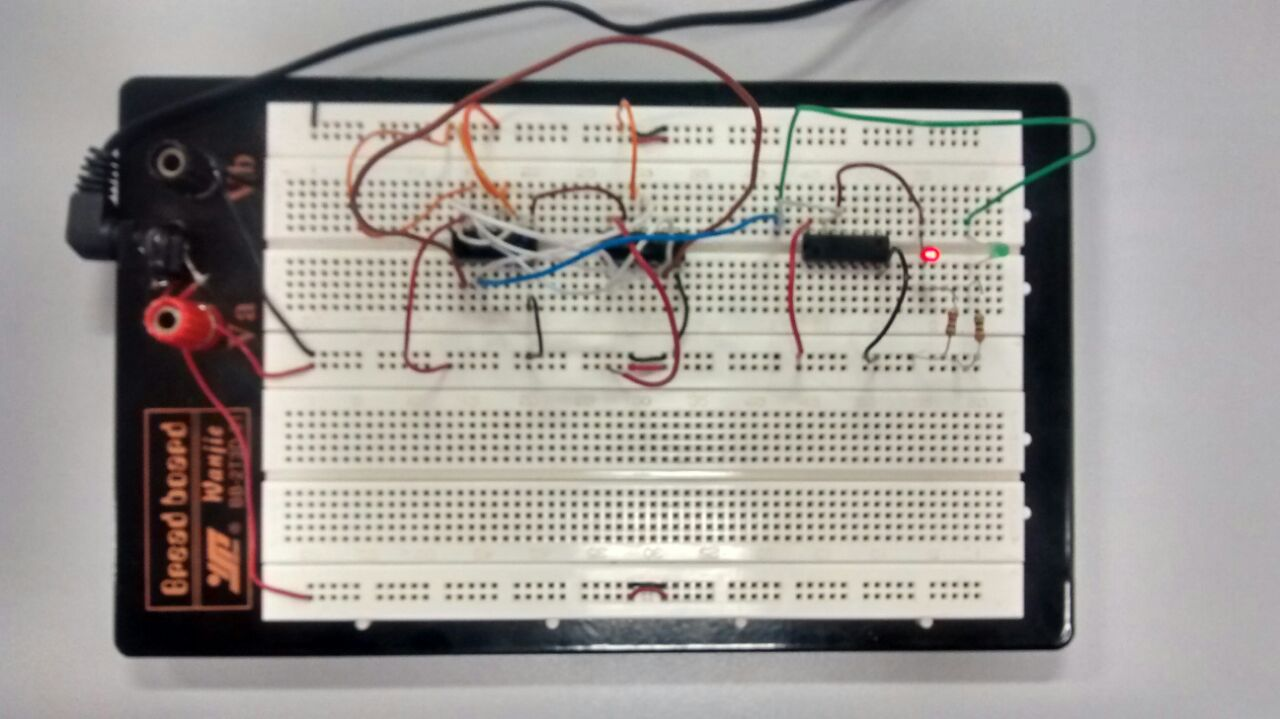
\includegraphics[width=1\textwidth]{img/cenario1/protoboard2}
	\end{figure}

\section{Cenario 2}
	Para a realização deste experimento, foram utilizados o programa Quartus 13.0 SP 1 e a placa \ac{fpga}
	Cyclone II - EP2C20F484C7.

	A partir do problema proposto, montou-se a seguinte expressão lógica
	$$ P + G + \sim V$$
	com P representando \textit{se a porta estiver aberta}, G
	\textit{se nível de gelo do congelador estiver acima do permitido} e V
	\textit{se o nível de gás do motor estiver adequado}, após a
	montagem da expressão, foi elaborada a \autoref{table:tabelaVerdade2}. Com esta tabela e a expressão lógica,
	elaborou-se o circuito, conforme a \autoref{fig:desenhoCircuito2}. Com tais informações, foi repassado o circuito
	para o Quartus, depois renomeou-se as entradas e saídas para que, por meio do arquivo tradutor, a placa
	\ac{fpga} reconhecesse os componentes.
	Para cobrir todos os casos de testes, foi realizada uma simulação, conforme a \autoref{fig:printSimulacao}.

	\begin{table}[h]
		\centering
		\caption{Tabela verdade da expressão lógica}\label{table:tabelaVerdade2}
		\begin{tabular}{c|c|c|c}
		%\hline
			\textbf{P} & \textbf{G} & \textbf{$\sim$V} & \textbf{P+G+($\sim$V)} \\
			\hline
			0 & 0 & 0 & 0\\\hline
			0 & 0 & 1 & 1\\\hline
			0 & 1 & 0 & 1\\\hline
			0 & 1 & 1 & 1\\\hline
			1 & 0 & 0 & 1\\\hline
			1 & 0 & 1 & 1\\\hline
			1 & 1 & 0 & 1\\\hline
			1 & 1 & 1 & 1
		\end{tabular}
	\end{table}

	\begin{figure}[H]
	    \centering
		\caption{\label{fig:desenhoCircuito2}Desenho do circuito}
		\includegraphics{img/cenario2/desenhoCircuito}
	\end{figure}


	\begin{figure}[H]
	    \centering
		\caption{\label{fig:printCircuito2}Imagem do circuinto no programa Quartus}
		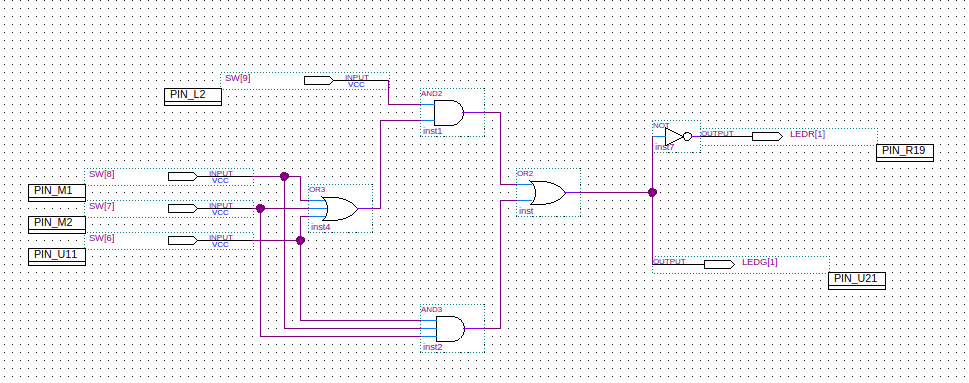
\includegraphics[width=1\textwidth]{img/cenario2/printCircuito}
	\end{figure}

	A porta SW[9] representa a P, a SW[8] representa a G, a SW[7]
	 representa a $\sim$V e a LEDR[1] é um led vermelho que irá
	 indicar o resultado provido da expressão lógica. Uma observação que não merece uma devida atenção é que
	 na \autoref{fig:desenhoCircuito2} foram necessárias a utilização de duas portas \textit{OR}, enquanto na
	 \autoref{fig:printCircuito2} foi necessária apenas a utilização de uma porta \textit{OR}. Isso ocorreu pelo fato
	 de que no Quartus existe a possibilidade de utilizar uma porta \textit{OR} de três entradas.

	Por fim, o circuito virtual foi compilado, conforme \autoref{fig:printCompilacao2}.

	\begin{figure}[H]
	    \centering
		\caption{\label{fig:printCompilacao2}Resultado da compilação do circuito}
		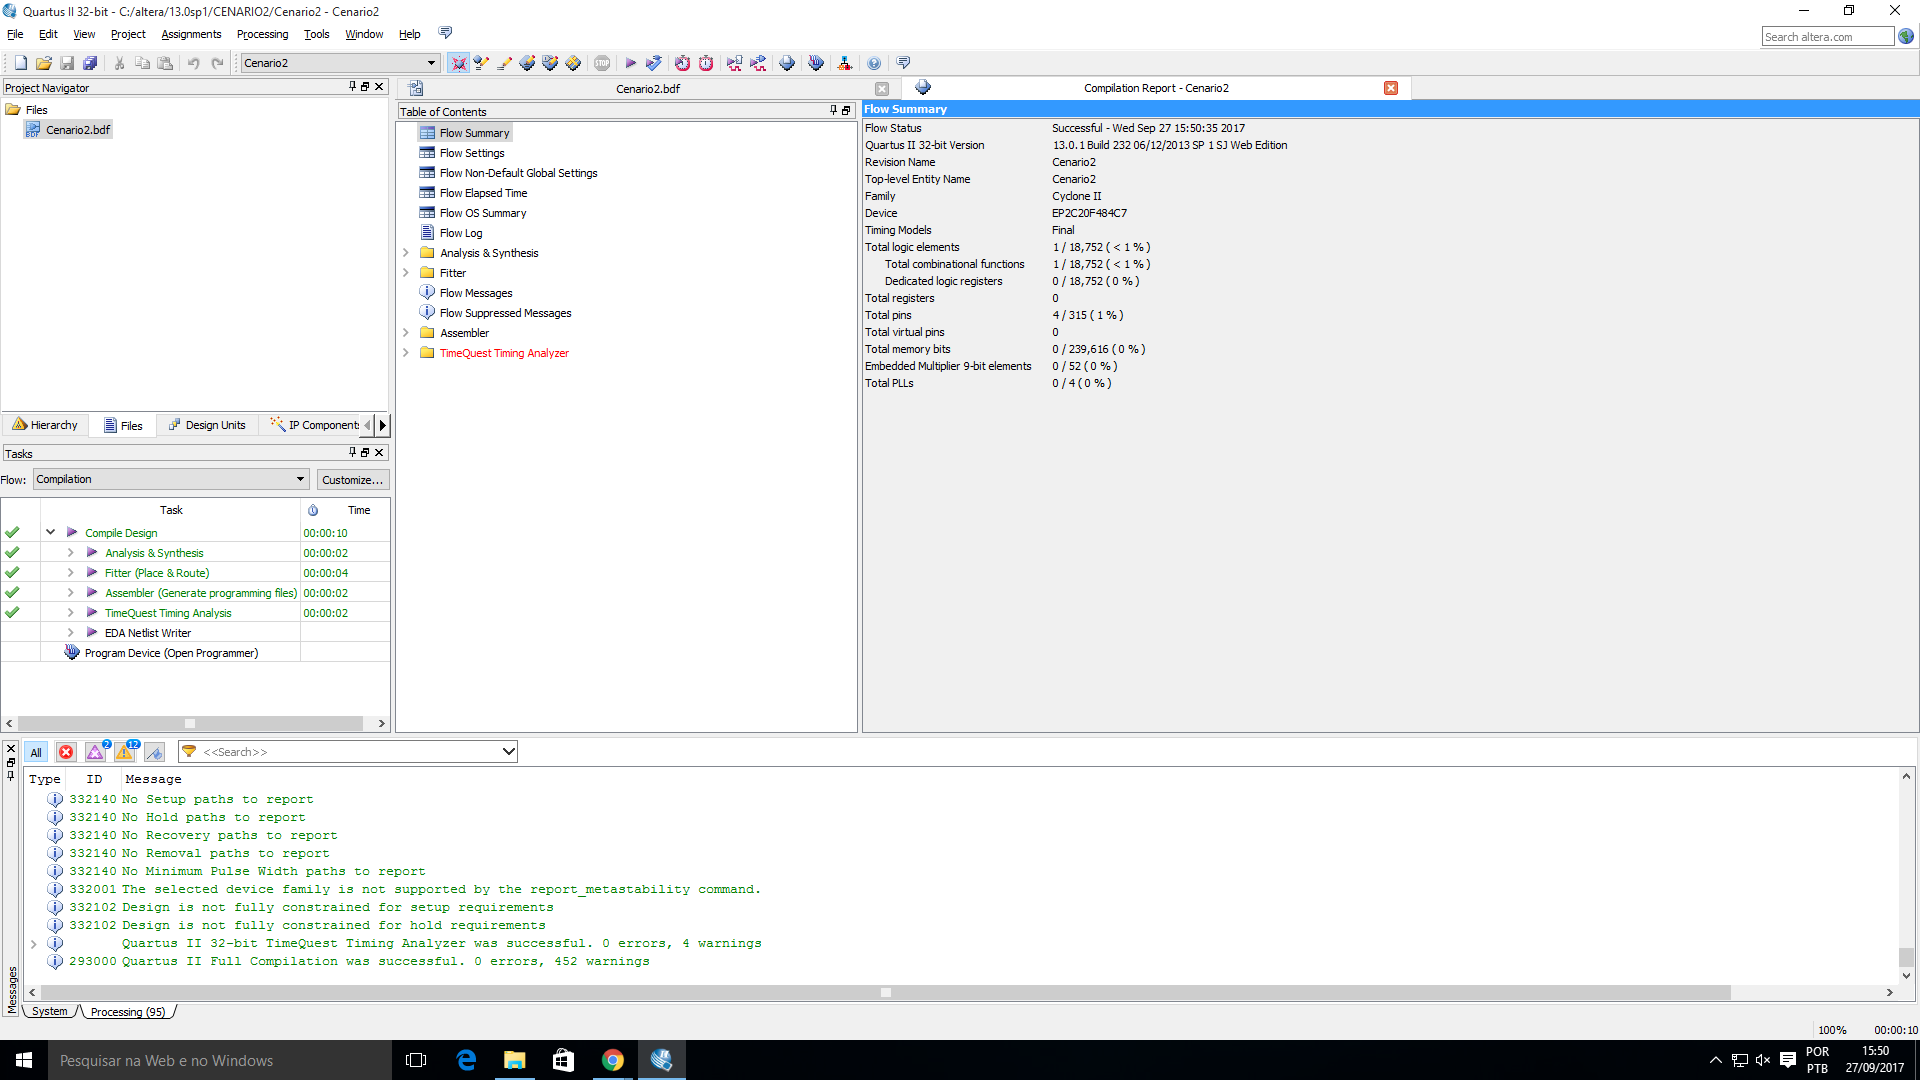
\includegraphics[width=1\textwidth]{img/cenario2/printCompilacao}
	\end{figure}


%Apresentar   o   detalhamento   da  execução  e   resultados   dos   passos   realizados
%durante   o   experimento,   incluindo   tabelas   verdade,   esquemáticos,   e   código
%(quando  houver).
%Especificar  componentes,  sistemas  e  instrumentos  utilizados.
%Usar listas, figuras e quadros, descrevê-los e discuti-los.

\chapter{Avaliação dos resultados do experimento}
	\section{ETAPA 1 – Display de 7 segmentos}

		Verificou-se, para todos os casos de entrada, que o valor previsto pela \autoref{table:tabelaVerdade1}
		como saída era válido, demonstrando sucesso na implementação do experimento. Isso pode
		ser visualizado tanto pela simulação, como na execução na placa.

		\begin{figure}[H]
		    \centering
			\caption{\label{fig:etapa1Simulacao}Resultado da simulação da etapa 1.}
			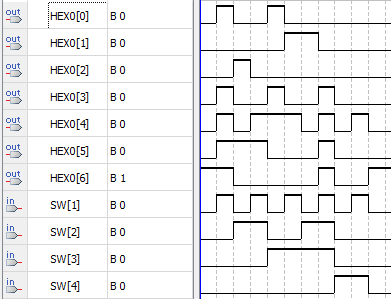
\includegraphics[width=1\textwidth]{img/etapa1/SimulacaoSegmentos7}
		\end{figure}

		\begin{figure}[H]
			\centering

			\begin{subfigure}[b]{0.44\textwidth}
				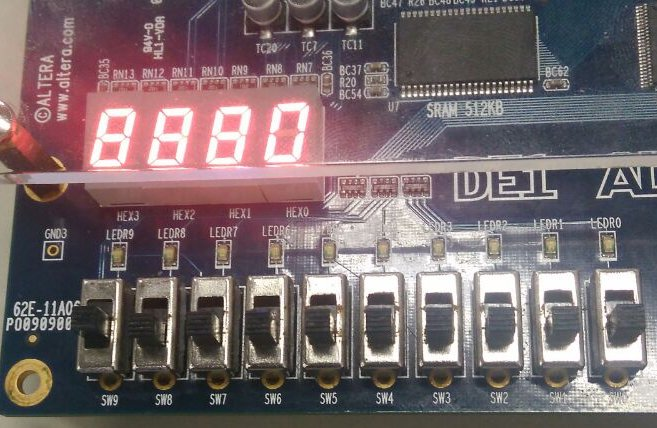
\includegraphics[width=\textwidth]{img/etapa1/0}
				\label{fig:etapa1-0}
				\caption{Número 0}
			\end{subfigure}
			~
			\begin{subfigure}[b]{0.44\textwidth}
				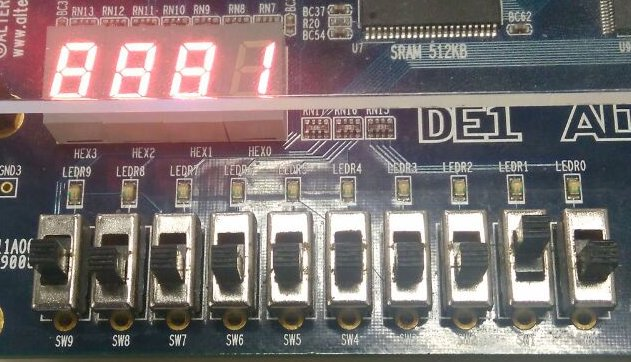
\includegraphics[width=\textwidth]{img/etapa1/1}
				\label{fig:etapa1-1}
				\caption{Número 1}
			\end{subfigure}

			\begin{subfigure}[b]{0.44\textwidth}
				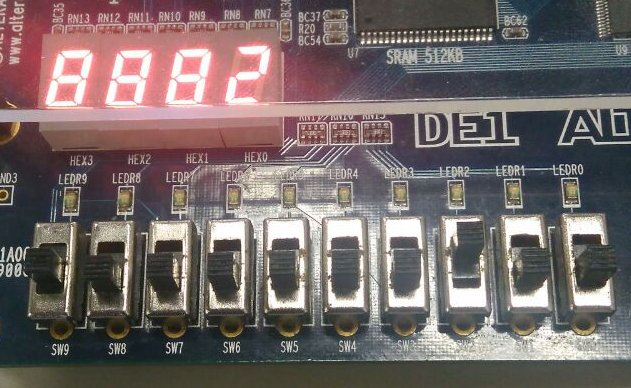
\includegraphics[width=\textwidth]{img/etapa1/2}
				\label{fig:etapa1-2}
				\caption{Número 2}
			\end{subfigure}
			~
			\begin{subfigure}[b]{0.44\textwidth}
				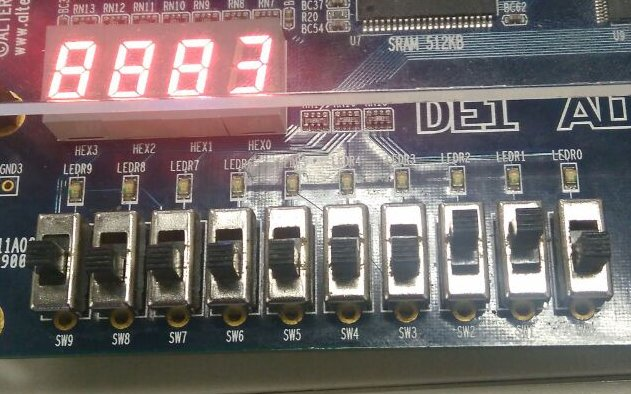
\includegraphics[width=\textwidth]{img/etapa1/3}
				\label{fig:etapa1-3}
				\caption{Número 3}
			\end{subfigure}
			\begin{subfigure}[b]{0.44\textwidth}
				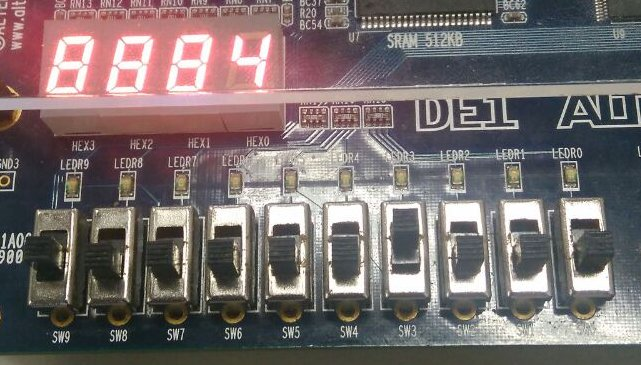
\includegraphics[width=\textwidth]{img/etapa1/4}
				\label{fig:etapa1-4}
				\caption{Número 4}
			\end{subfigure}
			~
			\begin{subfigure}[b]{0.44\textwidth}
				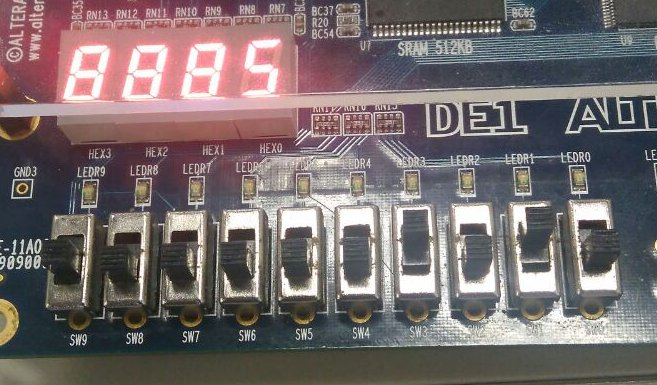
\includegraphics[width=\textwidth]{img/etapa1/5}
				\label{fig:etapa1-5}
				\caption{Número 5}
			\end{subfigure}

			\caption{Teste do circuito rodando na placa, no intervalo de 0-5.}\label{fig:etapa1Teste1}
		\end{figure}

		\begin{figure}[H]
			\centering

			\begin{subfigure}[b]{0.44\textwidth}
				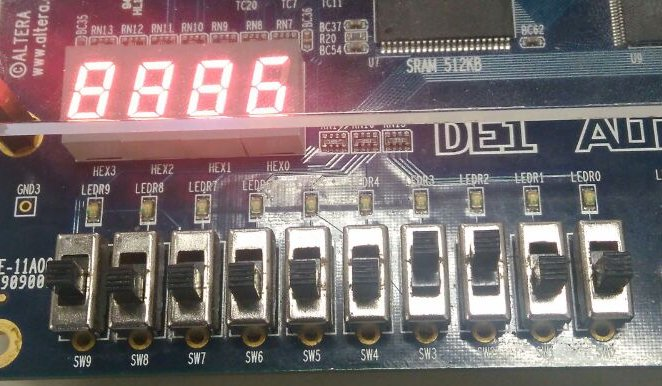
\includegraphics[width=\textwidth]{img/etapa1/6}
				\label{fig:etapa1-6}
				\caption{Número 6}
			\end{subfigure}
			~
			\begin{subfigure}[b]{0.44\textwidth}
				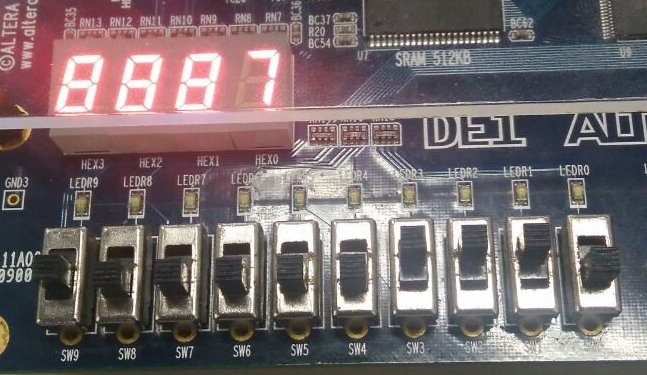
\includegraphics[width=\textwidth]{img/etapa1/7}
				\label{fig:etapa1-7}
				\caption{Número 7}
			\end{subfigure}

			\begin{subfigure}[b]{0.44\textwidth}
				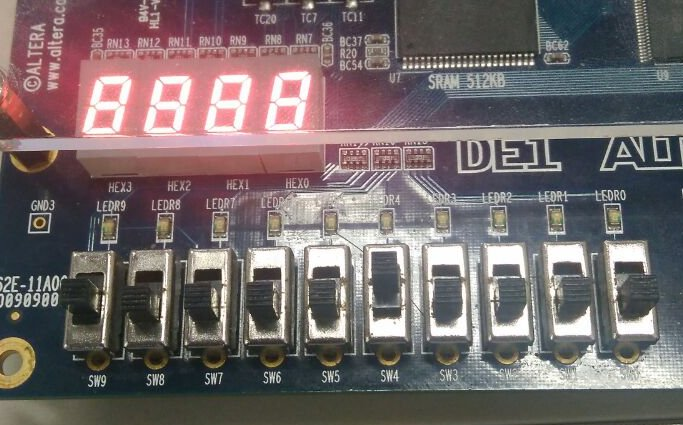
\includegraphics[width=\textwidth]{img/etapa1/8}
				\label{fig:etapa1-8}
				\caption{Número 8}
			\end{subfigure}
			~
			\begin{subfigure}[b]{0.44\textwidth}
				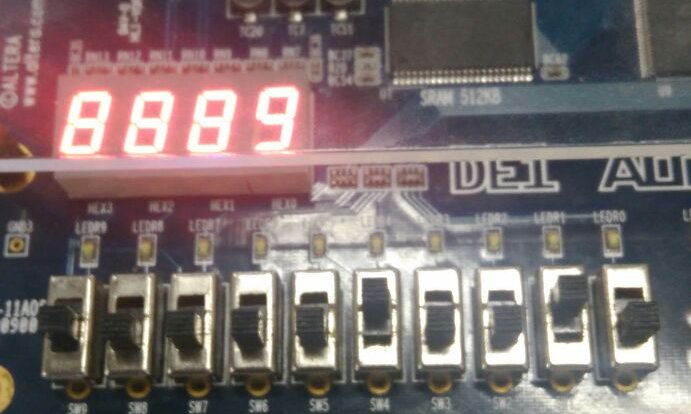
\includegraphics[width=\textwidth]{img/etapa1/9}
				\label{fig:etapa1-9}
				\caption{Número 9}
			\end{subfigure}

			\caption{Teste do circuito rodando na placa, no intervalo de 6-9.}\label{fig:etapa1Teste2}
		\end{figure}


	\section{ETAPA 2 – Meio-somador 1 bit}
		Na etapa 2, o experimento demonstrou os resultados esperados, de acordo com a
		 \autoref{table:tabelaMeioSomador}.

		\begin{figure}[H]
		    \centering
			\caption{\label{fig:etapa2Simulacao}Resultado da simulação da etapa 2.}
			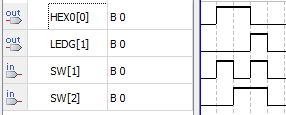
\includegraphics[width=1\textwidth]{img/etapa2/SimulacaoMeioSomador1Bit}
		\end{figure}

		Após o deploy na placa no kit DE1, o kit educacional da Altera, o circuito apresentou
		 os resultados esperados, representando o resultado da soma no display de 7 segmentos HEX0 ,
		e indicando a presença de um \textit{carry} ou não, através do LEDG[1],
		 conforme \autoref{fig:etapa2Teste}.

		\begin{figure}[H]
			\centering

			\begin{subfigure}[b]{0.44\textwidth}
				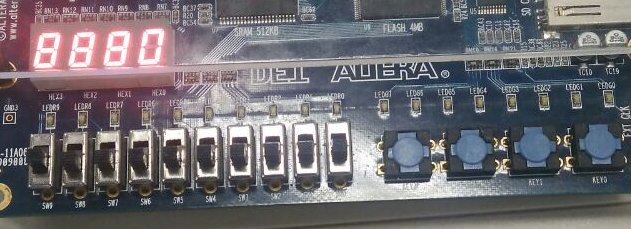
\includegraphics[width=\textwidth]{img/etapa2/00}
				\label{fig:etapa2-00}
				\caption{Entrada 0 0}
			\end{subfigure}
			~
			\begin{subfigure}[b]{0.44\textwidth}
				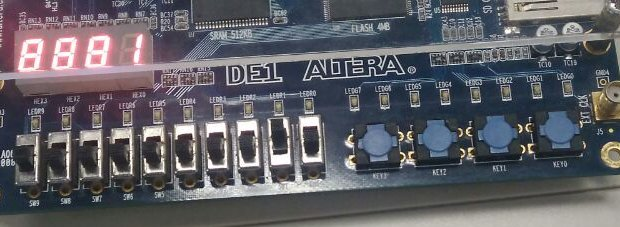
\includegraphics[width=\textwidth]{img/etapa2/01}
				\label{fig:etapa2-01}
				\caption{Entrada 0 1}
			\end{subfigure}

			\begin{subfigure}[b]{0.44\textwidth}
				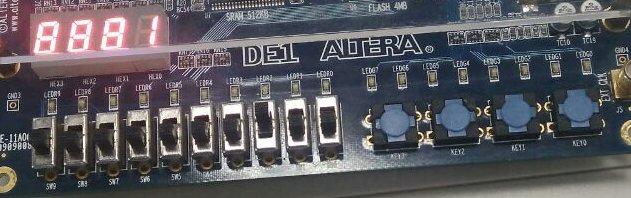
\includegraphics[width=\textwidth]{img/etapa2/10}
				\label{fig:etapa2-10}
				\caption{Entrada 1 0}
			\end{subfigure}
			~
			\begin{subfigure}[b]{0.44\textwidth}
				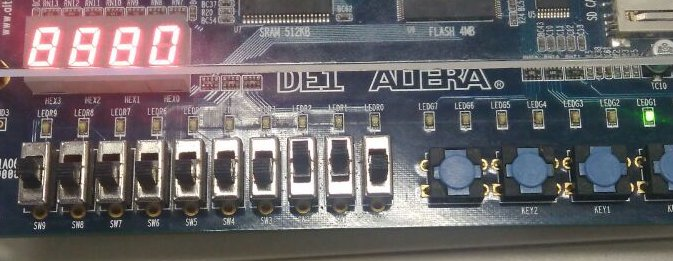
\includegraphics[width=\textwidth]{img/etapa2/11}
				\label{fig:etapa2-11}
				\caption{Entrada 1 1}
			\end{subfigure}

			\caption{Teste do circuito rodando na placa.}\label{fig:etapa2Teste}
		\end{figure}

		Veja o circuito no \autoref{apendice:CircuitoEtapa2}.
	\section{ETAPA 3 – Meio-somador 4 bits}


%Apresentar os resultados da simulação em software e da utilização do Kit DE1 e/ou
%protoboard. Utilizar figuras, descrevê-las e discuti-las.

\chapter{Análise crítica e discussão}
	\section{ETAPA 1 – Display de 7 segmentos}
		Teve-se dificuldade para entender que era necessário criar um circuito
		para para cada segmento do display e na leitura do resultado da simulação.
	\section{ETAPA 2 – Meio-somador 1 bit}
		Teve-se dificuldade de como implementar o meio-somador utilizando apenas as portas NAND.
	\section{ETAPA 3 – Meio-somador 4 bits}
		Teve-se dificuldade para dividir o resultado em dois \textit{display}.


%Apresentar  a  visão do  grupo  sobre  o  experimento,  apresentando  pontos  fáceis  e
%de  dificuldades  para  a  realização  do  mesmo.  Comente  se  os  resultados  obtidos
%representam  o  comportamento  esperado   do   grupo   para  o   circuito,   fazendo
%relação com o conteúdo teórico.

\chapter{Outras informações}

% exemplos de escrita LaTeX
	%\chapter{Exemplos \LaTeX}
% exemplo de como inserir uma referencia adicional no sumario
\addcontentsline{toc}{chapter}{Exemplos que devem ser lidos :-)}

Esse capítulo tem exemplos de escrita utilizando o \LaTeX  utilizando \abnTeX, é muito simples escrever em \textbf{negrito}, \emph{italico}, ....

Leia o \ac{faq} do \abnTeX : \href{url}{https://github.com/abntex/abntex2/wiki/FAQ}

Existem diversos tutoriais para uso de \LaTeX, se você está utilizando esse modelo não precisará se preocupar com muitos dos detalhes técnicos do \LaTeX  e cuidar somente do seu texto.

Escolha seu editor : \href{url}{https://en.wikipedia.org/wiki/Comparison\_of\_TeX\_editors}


\section{Detalhes textuais}

O documento é dividido em capítulos, e cada capítulo dividido em seções utilizando o \abnTeX você pode dividir seus documentos nos níveis a seguir:

\begin{itemize}
\item chapter (1);
\item section (1.1);
\item subsection (1.1.1);
\item subsubsection (1.1.1.1);
\item subsubsubsection (1.1.1.1.1).
\end{itemize}

Tenha em mente que normalmente se utiliza no máximo o nível \emph{subsection}.
Ao definir as divisões do seu trabalho utilizando as diretivas do \LaTeX, elas são automaticamente inseridas no sumário do documento.

\subsection{Caracteres Reservados}



Alguns caracteres são reservados no \LaTeX e por isso para utilizar esses caracteres é necessario utilizar uma forma diferenciada de escrita. É possivel utilizar a macro \emph{symbol} com o codigo ascii do caracter desejado.
\begin{itemize}
\item barra invertida : \textbackslash   \symbol{92}    $\backslash$;
\item til  :  \symbol{126} ;
\item cifrão : \$;
\item sublinhado, \emph{underscore}, \emph{underline} : \_;
\item chaves : \} \{.
\end{itemize}



\subsection{Listas}

Em uma lista de itens cada item deve ser terminado por ponto e virgula, exceto o ultimo item que deve ter um ponto final.

\begin{itemize}
\item item 1;
\item item 2;
\item item ..;
\item item final.
\end{itemize}

\subsection{Elementos não textuais}

Elementos não textuais são aqueles que auxiliam o entendimento, não podem ficar "jogados" no texto, devem ser citados, cada elemento deve ser identificado por um \emph{label} único que permite a sua referencia, no texto utilizando \emph{ref} ou \emph{autoref}, esses elementos quando definidos corretamente também são inseridos nas listas presentes antes do sumário.


\subsection{Tabelas e Quadros}
A seção 3.32 da NBR14724:2011 define a Tabela como sendo uma "forma não discursiva de apresentar informações das quais o dado numérico se destaca como informação central" 

Quadros e tabelas são informações tabulares, mas Tabelas tem como objetivo apresentar números.

Uso de tabelas no \LaTeX : \href{url}{https://en.wikibooks.org/wiki/LaTeX/Tables}


\index{quadros}O \autoref{quadro-exemplo} é um exemplo de dados tabulares gerados em 
\LaTeX.

\begin{quadro}[htb]
\centering
\ABNTEXfontereduzida
\caption[Níveis de investigação]{Níveis de investigação.}
\label{quadro-exemplo}
\begin{tabular}{|p{2.6cm}|p{6.0cm}|p{2.25cm}|p{3.40cm}|}
  \hline
   \textbf{Nível de Investigação} & \textbf{Insumos}  & \textbf{Sistemas de Investigação}  & \textbf{Produtos}  \\
    \hline
    Meta-nível & Filosofia\index{filosofia} da Ciência  & Epistemologia &
    Paradigma  \\
    \hline
    Nível do objeto & Paradigmas do metanível e evidências do nível inferior &
    Ciência  & Teorias e modelos \\
    \hline
    Nível inferior & Modelos e métodos do nível do objeto e problemas do nível inferior & Prática & Solução de problemas  \\
   \hline
\end{tabular}
\legend{Fonte: Próprio Autor}
\end{quadro}



\index{tabelas}Já a \autoref{tab-exemplo} foi criada conforme o padrão do IBGE
requerido pelas normas da ABNT para documentos técnicos e acadêmicos. Números devem ser alinhados a direita.

\begin{table}[htb]
\centering
\caption{Um Exemplo de tabela}
\label{tab-exemplo}
\begin{tabular}{p{2.6cm}|r|r|r}
    \hline
   \textbf{Item} & \textbf{Janeiro}  & \textbf{Fevereiro}  & \textbf{Março}  \\
    \hline
    Classes & 2  & 10 & 20  \\
    \hline
    Linhas & 100  & 250 & 543 \\
    \hline
\end{tabular}
\fonte{Dados do Projeto}
\end{table}

\def\equationautorefname~#1\null{%
  Equação~(#1)\null
}


\index{equação}\index{Pitagoras}A \autoref{eq-pythagoras} mostra que também é possivel escrever equações diretamente em \LaTeX

\begin{equation}\label{eq-pythagoras}
a^2+b^2=c^2\,.
\end{equation}






% ---
\subsection{Figuras}
% ---

\index{figuras}Figuras podem ser criadas diretamente em \LaTeX,
como o exemplo da \autoref{fig_circulo}, ou inseridas a partir de arquivos externos como a \autoref{fig_logo}, que é o Logotipo do IFSP\index{IFSP}. \index{logotipo}

\begin{figure}[htb]
	\begin{center}
	    \setlength{\unitlength}{5cm}
		\begin{picture}(1,1)
		\put(0,0){\line(0,1){1}}
		\put(0,0){\line(1,0){1}}
		\put(0,0){\line(1,1){1}}
		\put(0,0){\line(1,2){.5}}
		\put(0,0){\line(1,3){.3333}}
		\put(0,0){\line(1,4){.25}}
		\put(0,0){\line(1,5){.2}}
		\put(0,0){\line(1,6){.1667}}
		\put(0,0){\line(2,1){1}}
		\put(0,0){\line(2,3){.6667}}
		\put(0,0){\line(2,5){.4}}
		\put(0,0){\line(3,1){1}}
		\put(0,0){\line(3,2){1}}
		\put(0,0){\line(3,4){.75}}
		\put(0,0){\line(3,5){.6}}
		\put(0,0){\line(4,1){1}}
		\put(0,0){\line(4,3){1}}
		\put(0,0){\line(4,5){.8}}
		\put(0,0){\line(5,1){1}}
		\put(0,0){\line(5,2){1}}
		\put(0,0){\line(5,3){1}}
		\put(0,0){\line(5,4){1}}
		\put(0,0){\line(5,6){.8333}}
		\put(0,0){\line(6,1){1}}
		\put(0,0){\line(6,5){1}}
		\end{picture}
	\end{center}
	\caption{\label{fig_circulo}A delimitação do espaço}
	\legend{Fonte: os autores}
\end{figure}


\begin{figure}[htb]
    \centering
	
\includegraphics{\ifspprefixo/LogoUFSCar.jpg}
	\caption{\label{fig_logo}Logo IFSP}
	\legend{Fonte: IFSP}
\end{figure}





	%% ---
% Conclusão (outro exemplo de capítulo sem numeração e presente no sumário)
% ---
\chapter*[Conclusão]{Conclusão}
\addcontentsline{toc}{chapter}{Conclusão}
% ---

\lipsum[31-33]


% ----------------------------------------------------------
% Finaliza a parte no bookmark do PDF
% para que se inicie o bookmark na raiz
% e adiciona espaço de parte no Sumário
% ----------------------------------------------------------
\phantompart

% ----------------------------------------------------------
% ELEMENTOS PÓS-TEXTUAIS
% ----------------------------------------------------------
\postextual
% ----------------------------------------------------------

% ----------------------------------------------------------
% Referências bibliográficas
% ----------------------------------------------------------
\bibliography{referencias,exemplos/abntex2-doc-abnt-6023}

%% ----------------------------------------------------------
% Glossário
% ----------------------------------------------------------
%
% Consulte o manual da classe abntex2 para orientações sobre o glossário.
%
\glossary
\printglossaries

% ----------------------------------------------------------
% Apêndices
% ----------------------------------------------------------

% ---
% Inicia os apêndices
% ---
\begin{apendicesenv}

% Imprime uma página indicando o início dos apêndices
\partapendices

\chapter{Imagem do circuito para a representação de um número de 4 \textit{bits} em um display de 7 segmentos}
	\label{apendice:CircuitoEtapa1}
	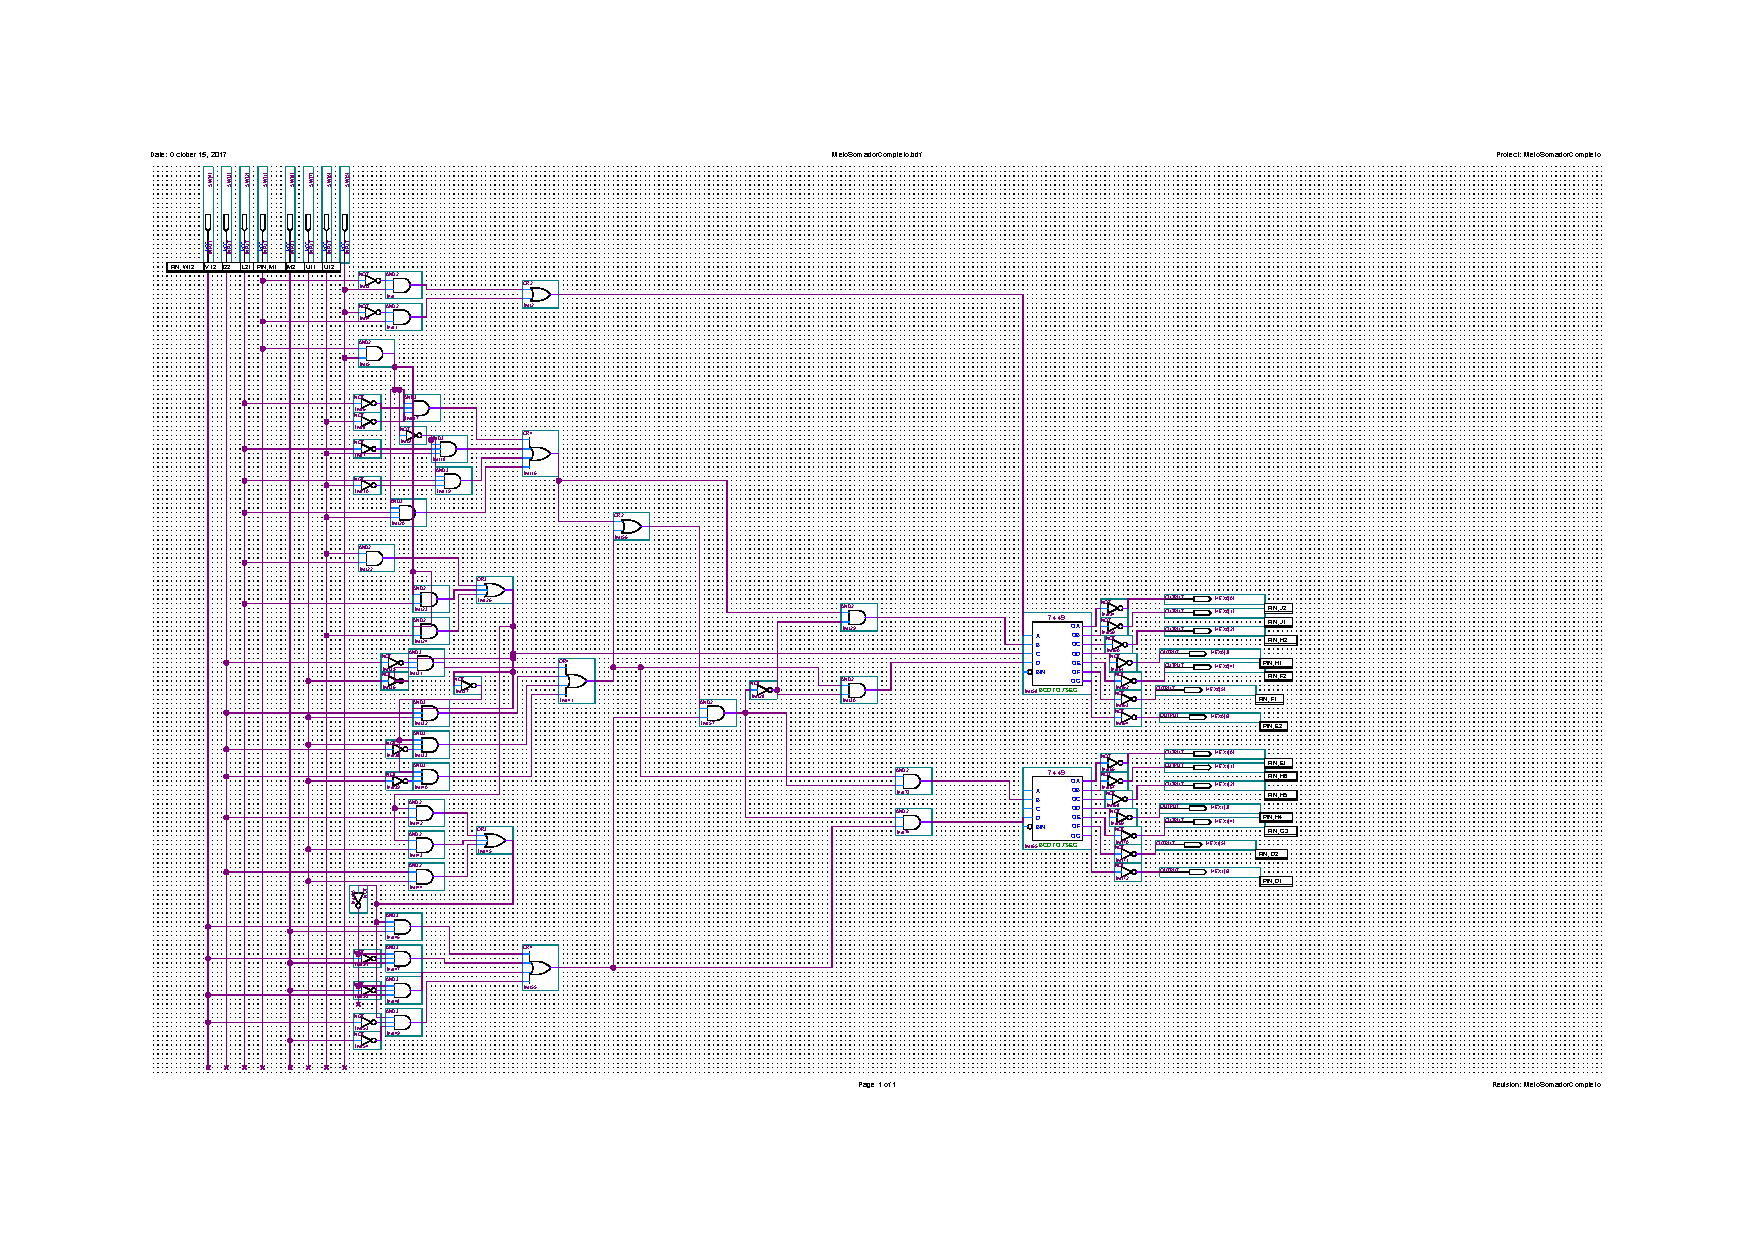
\includepdf[pages=1,landscape,frame=false]{apendices/MeioSomadorCompleto.pdf}

\chapter{Imagem do circuito do meio-somador de 4 \textit{bits}}
	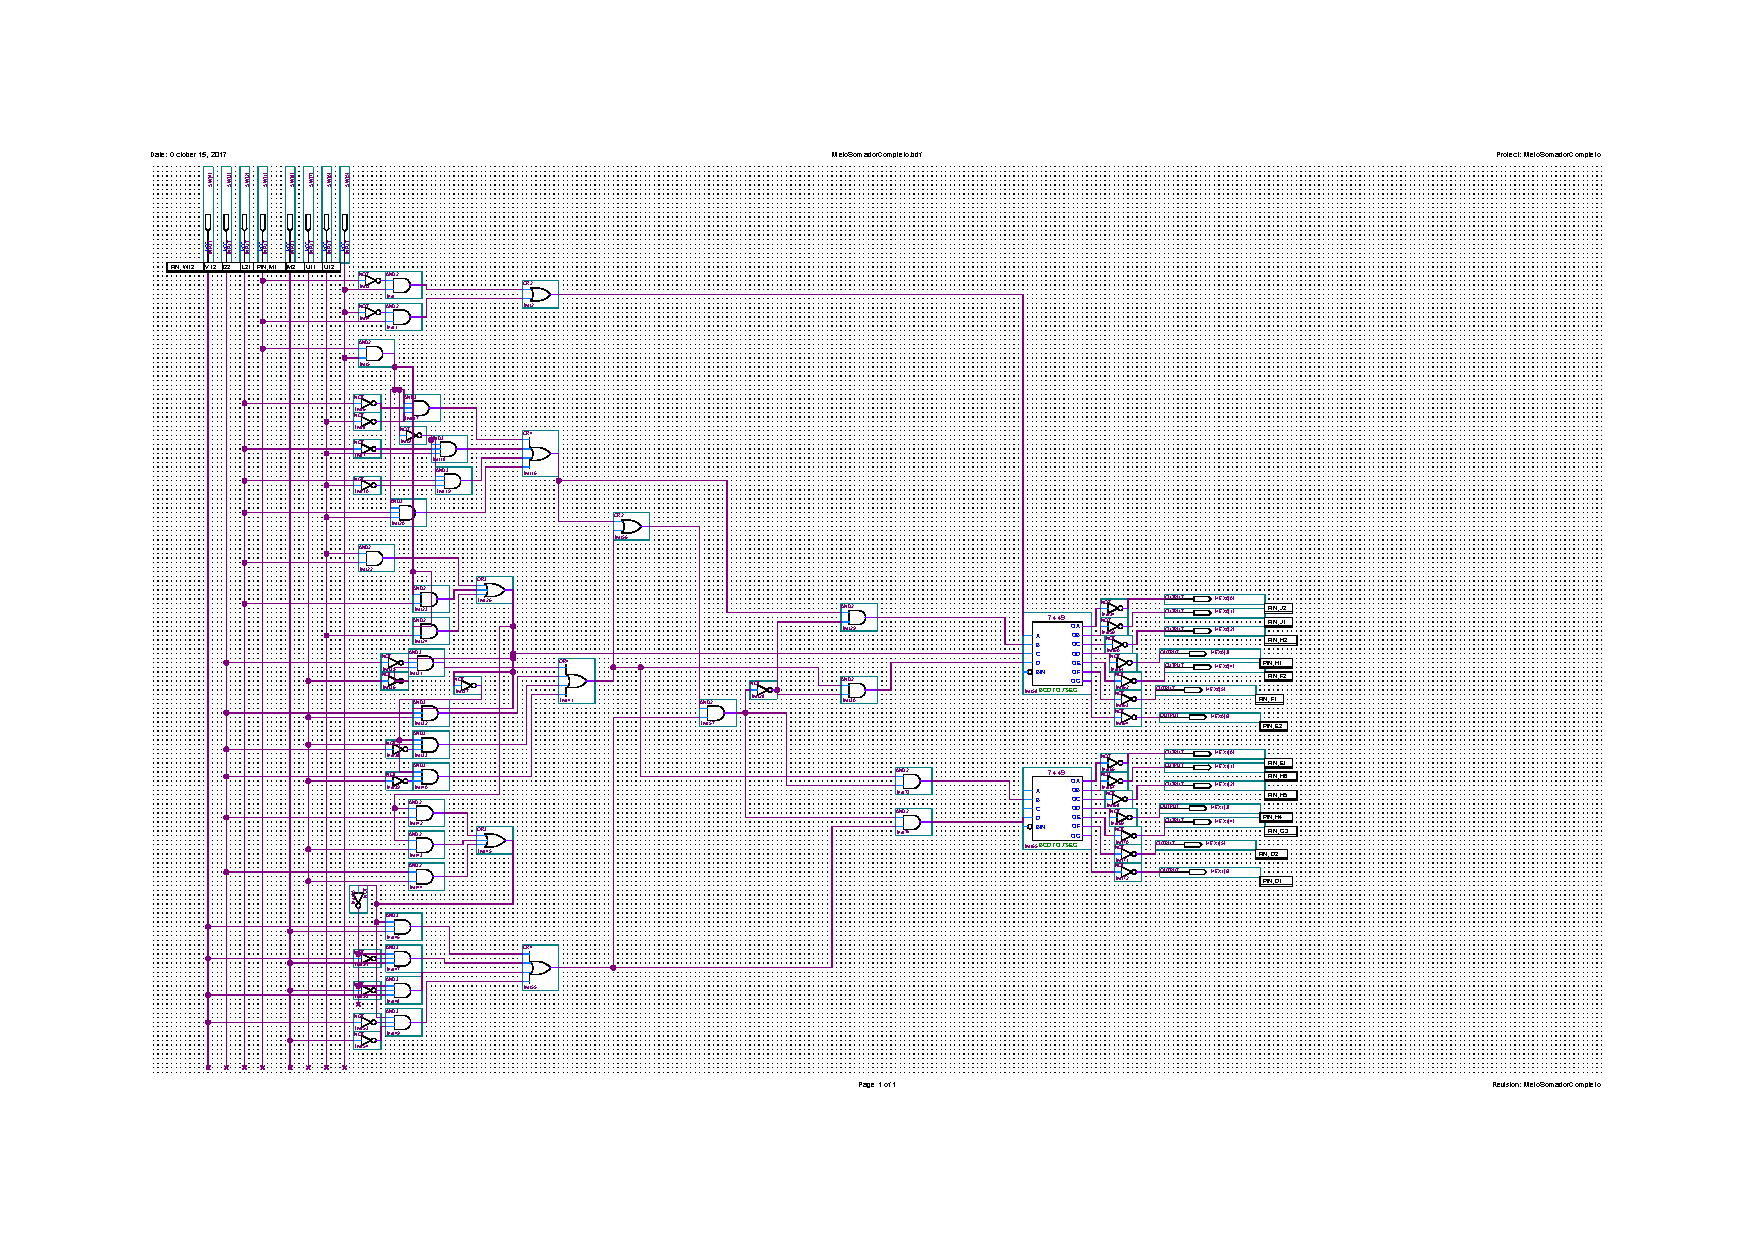
\includepdf[pages=1,landscape,frame=false]{apendices/MeioSomadorCompleto.pdf}



\end{apendicesenv}
% ---

% ----------------------------------------------------------
% Anexos
% ----------------------------------------------------------

% ---
% Inicia os anexos
% ---
\begin{anexosenv}

% Imprime uma página indicando o início dos anexos
\partanexos

% ---
\chapter{Manual pdfpages(parcial)}
% ---
\index{pdf}
% somente algumas páginas
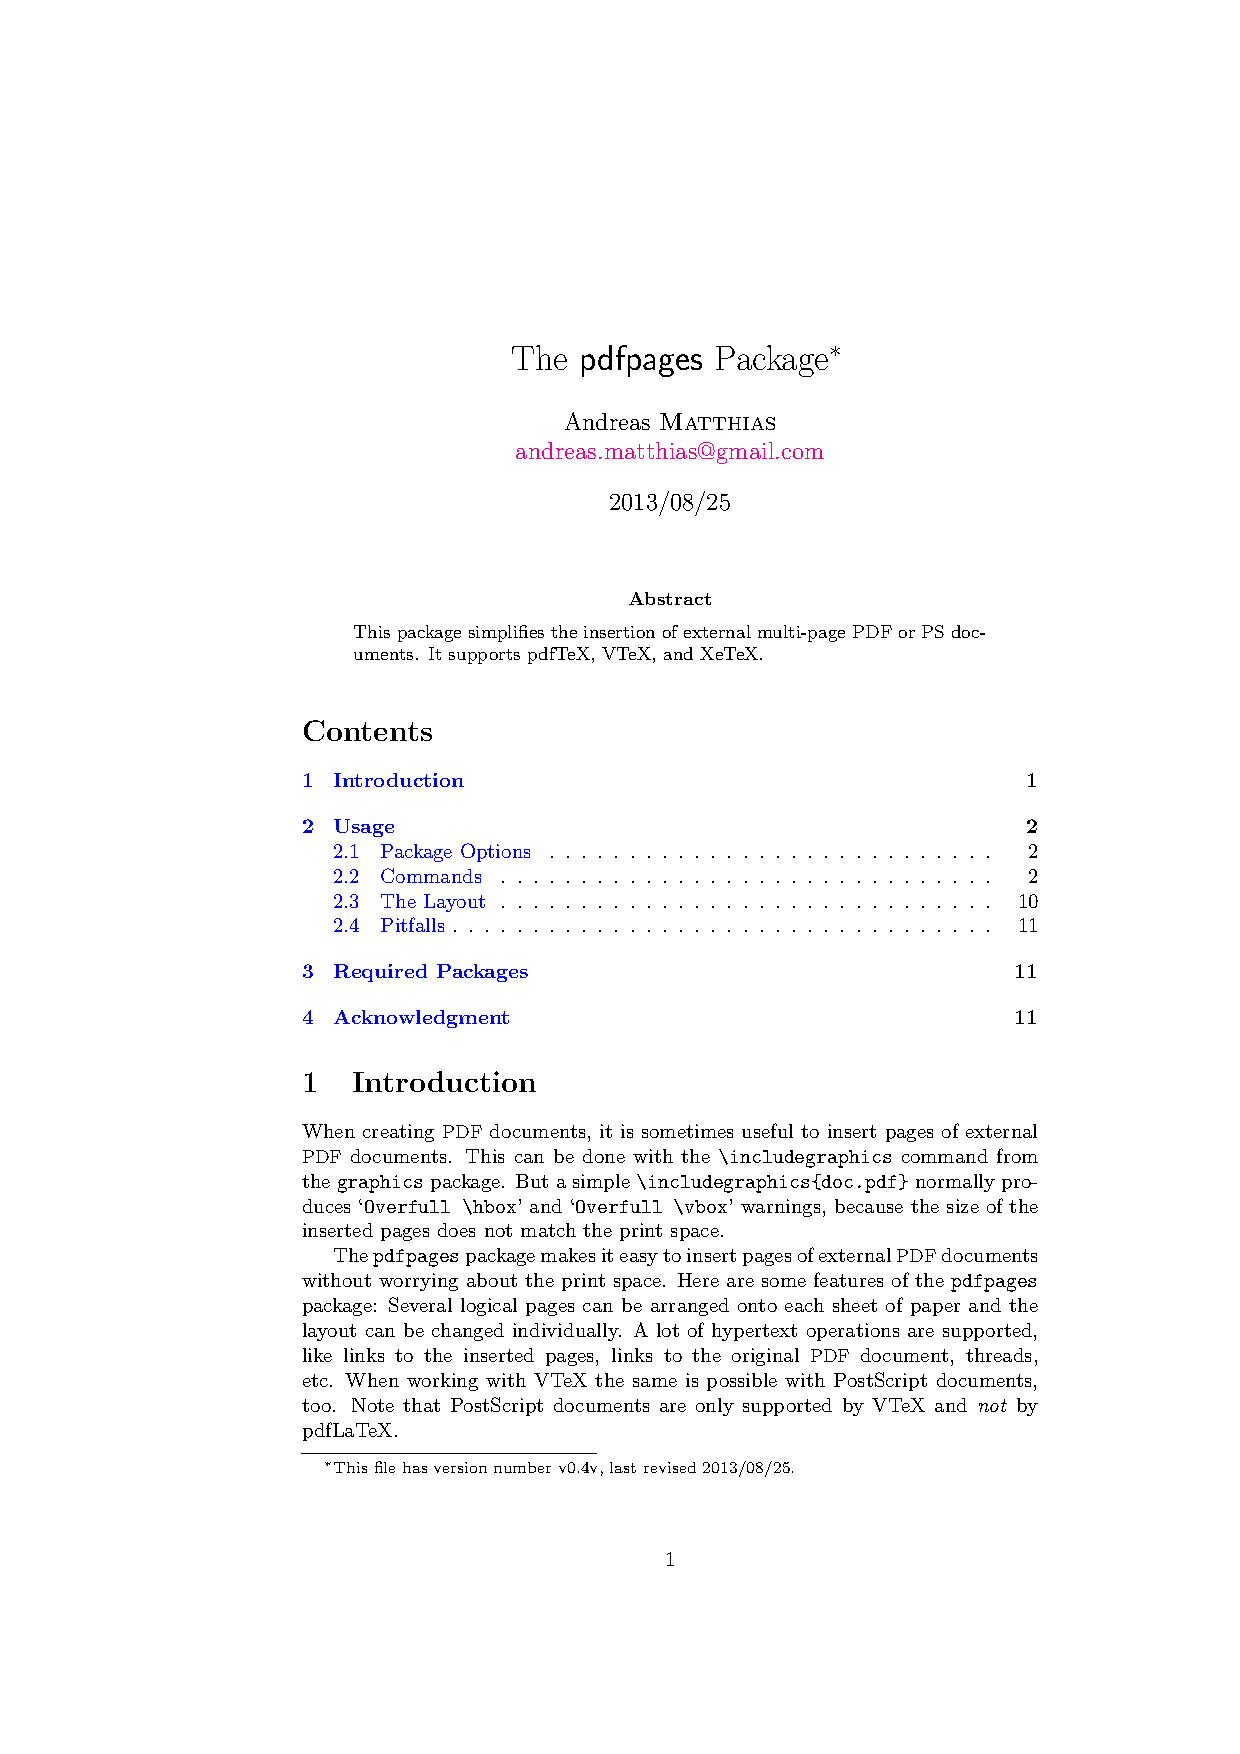
\includepdf[pages=1-3,frame=false]{anexos/pdfpages.pdf}


\end{anexosenv}



%---------------------------------------------------------------------
% INDICE REMISSIVO - Quando necessário
% As palavras indexadas devem ser definidas com \index{} no texto
%---------------------------------------------------------------------
\phantompart
	%\printindex

%---------------------------------------------------------------------

\end{document}
